\documentclass[handout]{beamer}

\usepackage{Haust2017glærur}

\title{Stærðfræðimynstur í tölvunarfræði}
\subtitle{Vika 13, seinni fyrirlestur}

\begin{document}

\begin{frame}
\titlepage
\end{frame}


\section{Inngangur}

\begin{frame}{Í síðasta tíma}
    \begin{itemize}
        \item Spanntré
        \item Dýptarleit og breiddarleit
        \item Léttustu spanntré
        \begin{itemize}
            \item Reiknirit Prims og Kruskals
        \end{itemize}
    \end{itemize}
\end{frame}

\section{Endanlegar stöðuvélar}

\begin{frame}{Endanlegar stöðuvélar}
\begin{itemize}
 \item Hægt er að lýsa ýmsum vélum og forritum með því að nota endanlega stöðuvél (e. \emph{finite-state machine})
 \item Grundvallaratriði í stöðuvélum er hugmyndin um að útreikningum eða aðgerðum megi lýsa með ástöndum (e. \emph{state}) og færslum þeirra á milli
 \item Dæmi: Læst hringhlið í skemmtigarði
\end{itemize}
\begin{center}
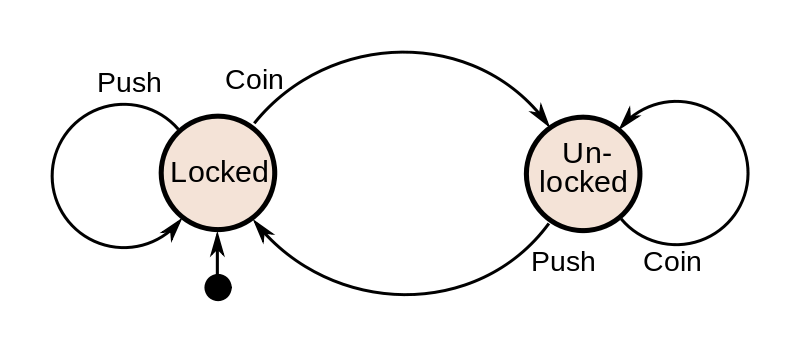
\includegraphics[width=0.5\textwidth]{turnstile-machine}
\end{center}
\end{frame}

\begin{frame}{Hagnýtingar}
\begin{itemize}
 \item Stöðuvélar og hugmyndir sem á þeim byggja koma mjög víða við
  \begin{itemize}
  \item Þýðendur og túlkar
  \item Reglulegar segðir
  \item Textagreining
  \item Tölvuleikir
 \end{itemize}
 \item Hjálpa til við að skipuleggja virkni forrita
 \item Notaðar í tölvunarfræði til formlegrar framsetningar á ``forritum''
\end{itemize}
\end{frame}

\section{Endanlegar stöðuvélar án úttaks}

\begin{frame}{Samþykkjarar}
Hægt er að nota stöðuvélar til að samþykkja strengi eða hafna þeim. Köllum slíkar vélar endanlega samþykkjara (e. \emph{acceptors}, í bók fjallað um sem \emph{finite-state automata}).

\begin{center}
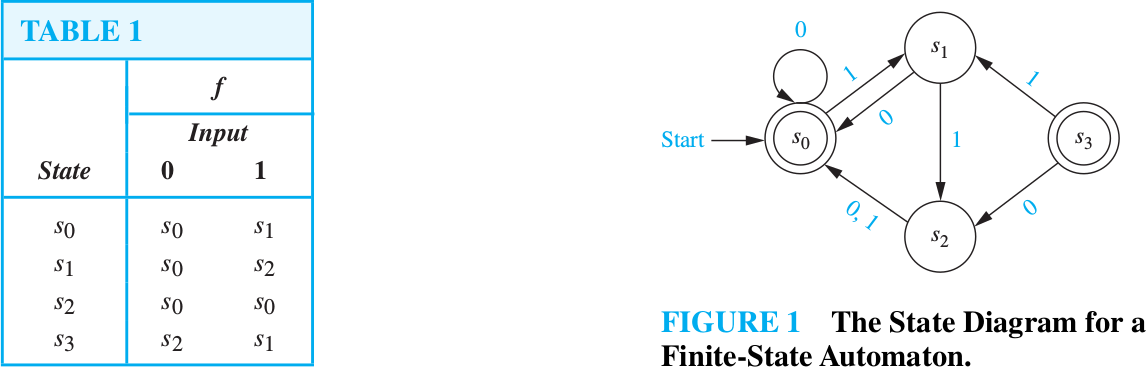
\includegraphics[width=0.95\textwidth]{dfa-example1}
\end{center}
\end{frame}

\begin{frame}{Samþykkjarar}
    \begin{tcolorbox}[title=Samþykkjarar]
        Endanlegur samþykkjari $M = (S, I , f, s_0, F)$ samanstendur af:
        \begin{itemize}
            \item $S$, endanlegu mengi staða
            \item $I$, endanlegu inntaksstafrófi
            \item $f$, færslufalli sem varpar hverju pari af stöðu og inntaki í nýja stöðu (fallsgildi $f$ eru stöður)
            \item $s_0$, upphafsstöðu
            \item $F$, hlutmengi í $S$ sem táknar lokastöður
        \end{itemize}
    \end{tcolorbox}
    Þessi skilgreining á við löggengan (e. \emph{deterministic}) samþykkjara.
\end{frame}

\begin{frame}{Notkun skilgreiningarinnar}
    Oft látum við mynd af samþykkjara duga til að lýsa honum.
    \begin{center}
        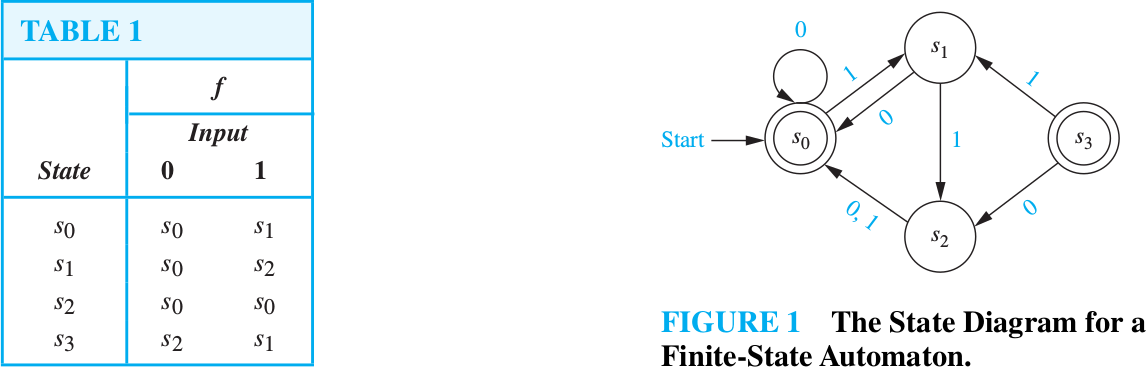
\includegraphics[width=0.95\textwidth]{dfa-example1}
    \end{center}
    Hér er $S=\{s_0, s_1,s_2,s_3\}$, $I = \{0,1\}$, $f$ skilgreint með töflu, $s_0$ er samnefnt og $F=\{s_0, s_3\}$.
\end{frame}

\begin{frame}{Mál og samþykkjarar}
\begin{tcolorbox}
Strengur $x$ er samþykktur (e. \emph{accepted} eða \emph{recognized}) af samþykkjara $M$ taki hann $M$ úr upphafsstöðu yfir í lokastöðu.

Málið sem $M$ samþykkir (e. \emph{the language accepted by $M$}) er mengi allra strengja sem $M$ samþykkir.
\end{tcolorbox}
Tvær stöðuvélar eru sagðar jafngildar ef þær samþykkja sama mál.
\end{frame}

\begin{frame}{Skilgreiningar}
    \begin{itemize}
        \item Stafróf $V$ (e. \emph{alphabet} eða \emph{vocabulary}) er endanlegt, ekki-tómt mengi af táknum (e. \emph{symbols})
        \item Mengi allra endanlegra strengja mynduðum með táknum úr $V$ er táknað með $V^*$
        \item Mál yfir $V$ (e. \emph{language over $V$}) er hlutmengi í $V^*$
        \item Samskeyting $A$ og $B$, þar sem $A\subseteq V^*,B\subseteq V^*$ er táknuð með $AB$ og er mengi þeirra samskeyttu strengja $xy$ þar sem $x\in A$ og $y \in B$
        \begin{itemize}
            \item $A^n$ er samskeyting $A$ við sjálft sig $n$ sinnum
        \end{itemize}
        \item Kleene lokun $A$ (e. \emph{Kleene closure of $A$}) er táknuð með $A^*$ og er samskeyting 0 eða fleiri strengja úr $A$
    \end{itemize}
\end{frame}

\begin{frame}{Dæmi}
Hvaða mál samþykkir þessi vél?

\begin{center}
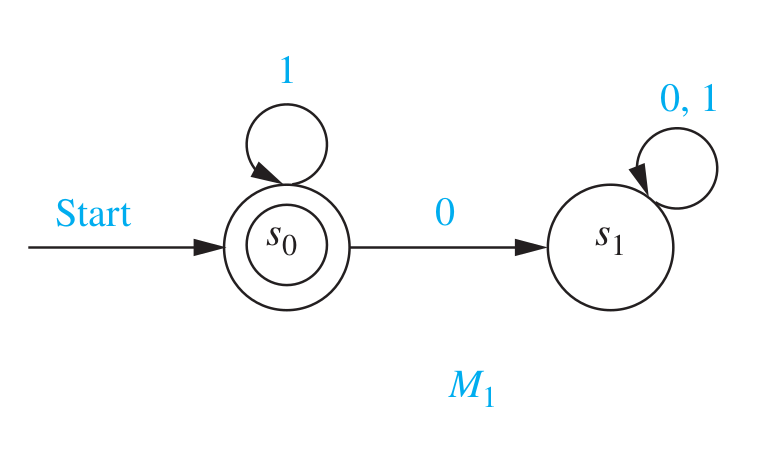
\includegraphics[width=0.6\textwidth]{dfa-example2}
\end{center}

\pause
Mál þeirra strengja sem eingöngu innihalda 0 eða fleiri ása.
\[
 L(M_1) = \{1^n | n \in 0, 1, 2, \ldots \}
\]

\end{frame}

\begin{frame}{Dæmi}
Hvaða mál samþykkir þessi vél?

\begin{center}
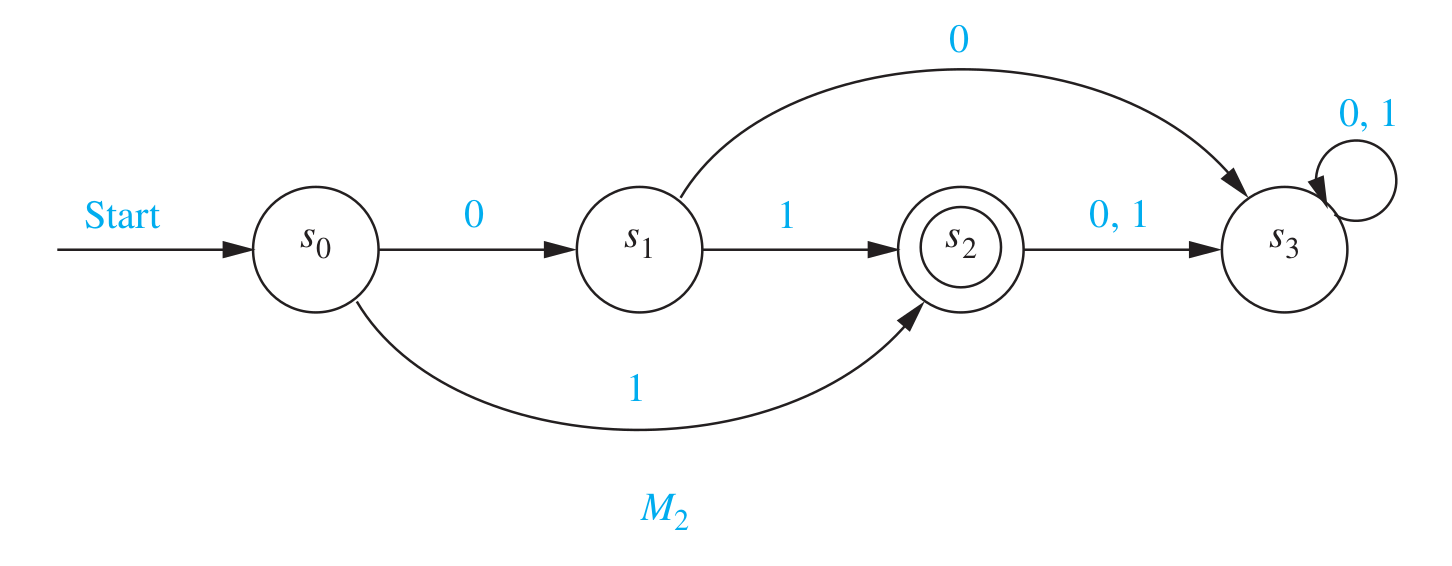
\includegraphics[width=\textwidth]{dfa-example3}
\end{center}

\pause
Við höfum nákvæmlega tvær leiðir til að komast í lokastöðu.
\[
 L(M_2) = \{1,01\}
\]

\end{frame}

\begin{frame}{Dæmi}
    \begin{itemize}
        \item Getum við búið til stöðuvélar (samþykkjara) sem samþykkja eftirfarandi mál?
        \begin{enumerate}[a)]
            \item Mengi bitastrengja sem byrja á 00
            \item Mengi bitastrengja sem innihalda 00
            \item Mengi bitastrengja sem innihalda ekki 00
            \item Mengi bitastrengja sem enda ekki á 00
            \item Mengi bitastrengja sem innihalda a.m.k. tvö 0
        \end{enumerate}
        \item Margar lausnir mögulegar, tvær stöðuvélar eru jafngildar ef þær samþykkja sama mál
    \end{itemize}
\end{frame}

\begin{frame}{Lausnir}
    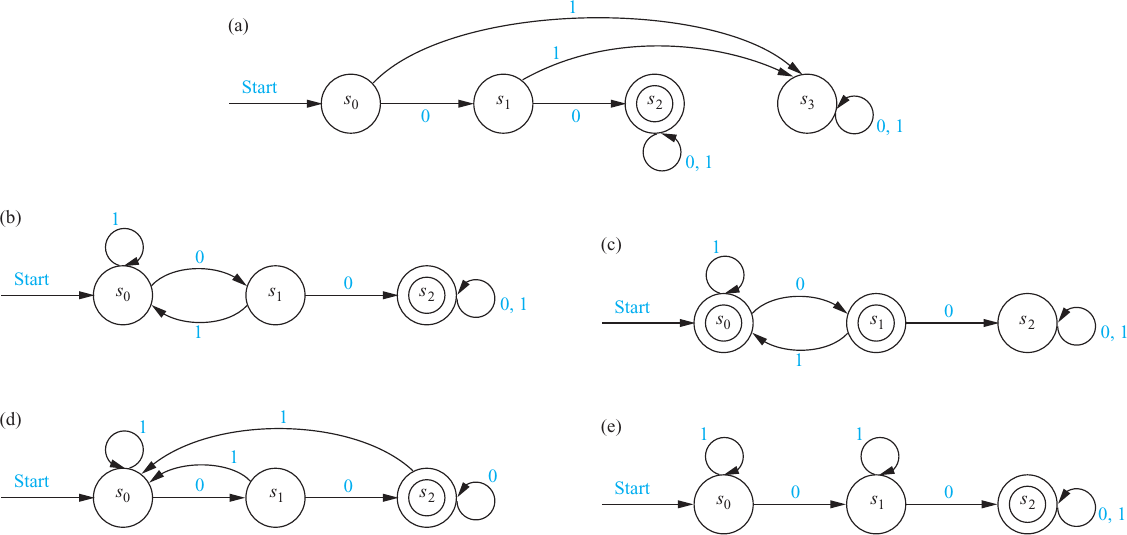
\includegraphics[width=\textwidth]{dfa-examples}
\end{frame}

\section{Löggengni og brigðgengni}

\begin{frame}{Brigðgengni og löggengni}
    \begin{itemize}
        \item Þeir samþykkjarar sem við höfum skoðað hér hafa varpað öllum mögulegum stöðu-inntaks pörum í nákvæmlega eina aðra stöðu
        \begin{itemize}
            \item Slíkar stöðuvélar eru kallaðar löggengar endanlegar stöðuvélar
        \end{itemize}
        \item Gætum líka skilgreint vélar þar sem hvert stöðu-inntakspar getur leitt okkur í meira en eina mismunandi stöðu
        \item Algengar skammstafanir:
        \begin{itemize}
            \item DFA: Deterministic Finite Automaton
            \item NFA: Non-deterministic Finite Automaton
        \end{itemize}
    \end{itemize}
\end{frame}

\begin{frame}{Skilgreining}
    \begin{tcolorbox}[title=Brigðgengur samþykkjari]
        Endanlegur samþykkjari $M = (S, I , f, s_0, F)$ samanstendur af:
        \begin{itemize}
         \item $S$, endanlegu mengi staða
         \item $I$, endanlegu inntaksstafrófi
         \item $f$, færslufalli sem varpar hverju pari af stöðu og inntaki í \textbf{mengi af stöðum} ($f: S \times I \to P(S)$)
         \item $s_0$, upphafsstöðu
         \item $F$, hlutmengi í $S$ sem táknar lokastöður
        \end{itemize}
    \end{tcolorbox}
\end{frame}

\begin{frame}{Jafngildi}
    \begin{itemize}
        \item Löggengir og brigðgengir samþykkjarar eru jafn ``öflugir''
        \begin{itemize}
            \item Getum alltaf breytt brigðgengri vél í löggenga
            \begin{itemize}
                \item Fyrir $n$ stöðu brigðgenga vél gæti tilsvarandi löggeng vél þó innihaldið allt að $2^n$ stöður
            \end{itemize}
            \item Brigðgengar og löggengar vélar geta samþykkt sömu strengi
        \end{itemize}
    \end{itemize}
    \begin{tcolorbox}
        Sé málið $L$ samþykkt af brigðgenga endanlega samþykkjaranum $M_0$ þá er til löggengur endanlegur samþykkjari $M_1$ sem samþykkir $L$.
    \end{tcolorbox}
\end{frame}

\begin{frame}{Jafngildar vélar}
    \begin{columns}
        \column{0.4\textwidth}
        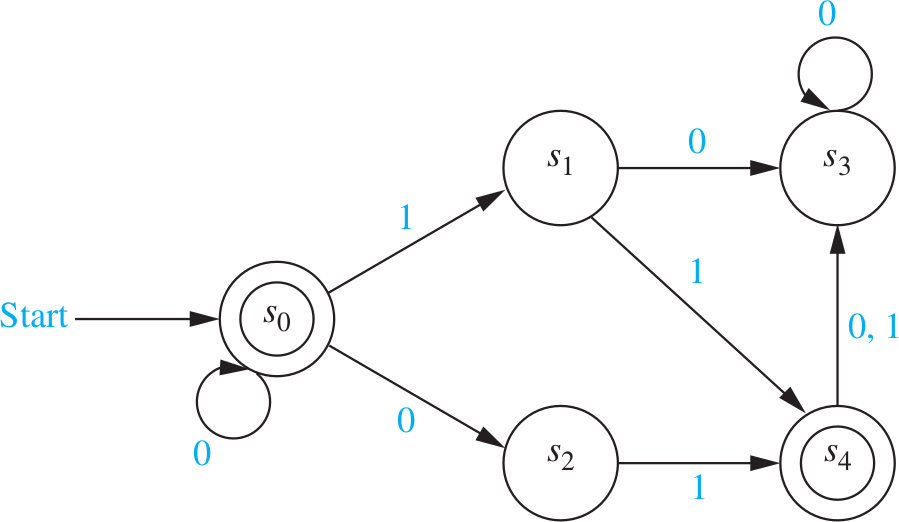
\includegraphics[width=\linewidth]{nfa-example}
        \pause
        \column{0.6\textwidth}
        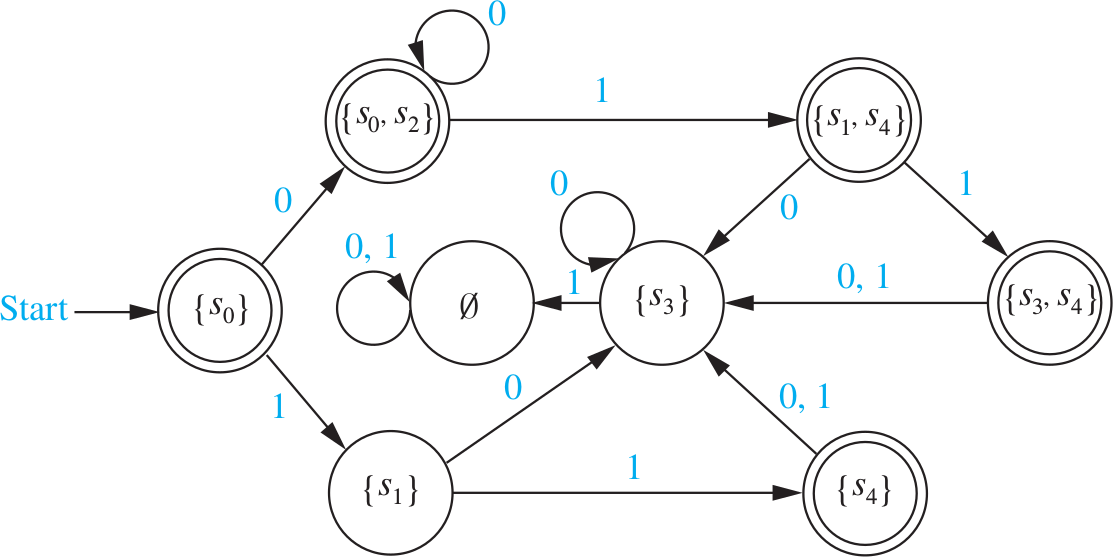
\includegraphics[width=\linewidth]{nfa-equiv}
    \end{columns}
    \pause
    \begin{center}
        Vélarnar samþykkja málið $\{0^n, 0^n01, 0^n11| n \geq 0\}$
    \end{center}
\end{frame}

\section{Reglulegar segðir}

\begin{frame}{Reglulegar segðir}
    \begin{itemize}
        \item Þeim málum sem reglulegir samþykkjarar geta samþykkt má lýsa með reglulegum segðum (e. \emph{regular expressions}).
        \item Möguleg skilgreining á reglulegri segð yfir mengi $I$:
        \begin{itemize}
            \item Tómi strengurinn er regluleg segð
            \item $x$ er regluleg segð þegar $x \in I$
            \item $(AB)$, $(A \cup B)$ og $A^*$ eru reglulegar segðir þegar $A$ og $B$ eru regulegar segðir
        \end{itemize}
        \item Nokkur blæbrigði eru til af reglulegum segðum í tölvum
    \end{itemize}
\end{frame}

\begin{frame}{Hagnýting reglulegra segða}
    \begin{itemize}
        \item Getum hugsað reglulegar segðir á tvenna vegu:
        \begin{itemize}
            \item Látum reglulegu segðina lýsa mengi
            \item Notum reglulega segð eins og samþykkjara
        \end{itemize}
        \item Hvaða mengjum lýsa eftirfarandi reglulegar segðir?
        \begin{itemize}
            \item $10^*$, $(10)^*$, $0 \cup 01$, $0(0 \cup 1)^*, (0^*1)^*$
        \end{itemize}
        \item Hvernig gætum við búið til reglulegar segðir fyrir
        \begin{itemize}
            \item Mengi bitastrengja með sléttum fjölda bita?
            \item Mengi bitastrengja sem endar á $0$ og inniheldur ekki $11$?
            \item Mengi bitastrengja sem inniheldur oddatölufjölda 0?
        \end{itemize}
    \end{itemize}
\end{frame}

\begin{frame}{Takmarkanir samþykkjara}
    \begin{itemize}
        \item Löggengir endanlegir samþykkjarar, brigðgengir endanlegir samþykkjarar og reglulegar segðir samþykkja sömu mengi
        \begin{itemize}
            \item Þetta eru regluleg mengi (e. \emph{regular sets})
        \end{itemize}
        \item Dæmi um mengi sem er ekki reglulegt: $\{0^n1^n| n\in \mathbf{N}\}$
        \item Þurfum öflugri líkön fyrir reiknanleika til að samþykkja slík mál
    \end{itemize}
\end{frame}

\begin{frame}{Næst}
Turing-vélar
\end{frame}


\end{document}
